\section{Background}\label{sec:relatedwork}

This syntax and explanation is a combination of ideas from from many sources \cite{Lyu2021,Li2020,Mei2006,Yu2005,Kruger2018}.

\subsection{Macroscopic Fluid Dynamics}

Traditionally, fluid dynamics problems are 
modelled by numerically solving some 
differential equations over the fluid's domain.
Fluid dynamics conserve mass, so solvers should account for the law of conservation of mass
\begin{align}
  \frac{\partial \rho}{\partial t} + \nabla \cdot (\rho \bm{u}) &= 0
\end{align}
where $\rho$ is density and $\bm{u}$ is velocity. 
Essentially, the change in density at any point should be 
balanced by mass entering or leaving that region.
Another common equation to account for is the Navier-Stokes momentum equation
\begin{align}
\frac{\partial}{\partial t} (\rho \bm{u}) 
+ \nabla \cdot (\rho \bm{u} \times \bm{u}) &= 
- \nabla \bm{p} + \nabla \cdot \sigma + F
\end{align}
where $\bm{p}$ is pressure, $\sigma$ is shear stress tensor, and $F$
represents any external forces like gravity. 
This is another conservation law that relates several \textit{macroscopic}
quantities of fluid.
Fluids dynamics are the emergent behavior of the \textit{microscopic} 
behavior of molecules.
Macroscopic quantities, like pressure, are an observed average of 
microscopic quantities.
Even fluid velocity, in the sense we're interested in, 
is a macroscopic quantity.

Many other approaches to modelling fluid dynamics,
like finite volume, finite element, and even 
smoothed particle hydrodynamics(?)
seek to solve for macroscopic 
fields like $\bm{u}$ and $\bm{p}$.

\subsection{LBM}
The lattice Boltzmann method (LBM) is a collection of techniques for
numerically modelling fluid dynamics that solves for microscopic quantities.
In particular, LBM solves the numerically solves 
the lattice Boltzmann equation
\begin{align}\label{eqn:cont_lbm}
  \frac{\partial f}{\partial t} + \bm{v} \cdot \nabla f = \Omega(f) + F\nabla_{\bm{v}} f
\end{align}
LBM solves this equation for a probability distribution $f(x, \bm{v}, t)$ which
describes the probability of a particle to be at point $x$, traveling with macroscopic velocity $\bm{v}$ at time $t$.

The discretization used in LBM to numerically solve \ref{eqn:cont_lbm} 
has two components.
First the fluid domain, space, is 
discretized onto a
grid of points $x \in \delta_x \mathbb{Z}^D$
where $\delta_x$ is the spacing between points in world coordinates
and $D$ is the spatial dimension ($3$ for most of our examples.)

The second part is discretizing the possible velocities a particle 
could be traveling in. 
Each point has a finite number, $Q$, of directions it can travel in, $c_i$.
These directions relate points in the grid and form the titular lattice.
These lattices are typically denoted by $D\#Q\#$.
Common lattices include $D2Q9$ (a) or $D3Q27$ (b), see below (figure from \cite{Li2020}.)
\begin{center}
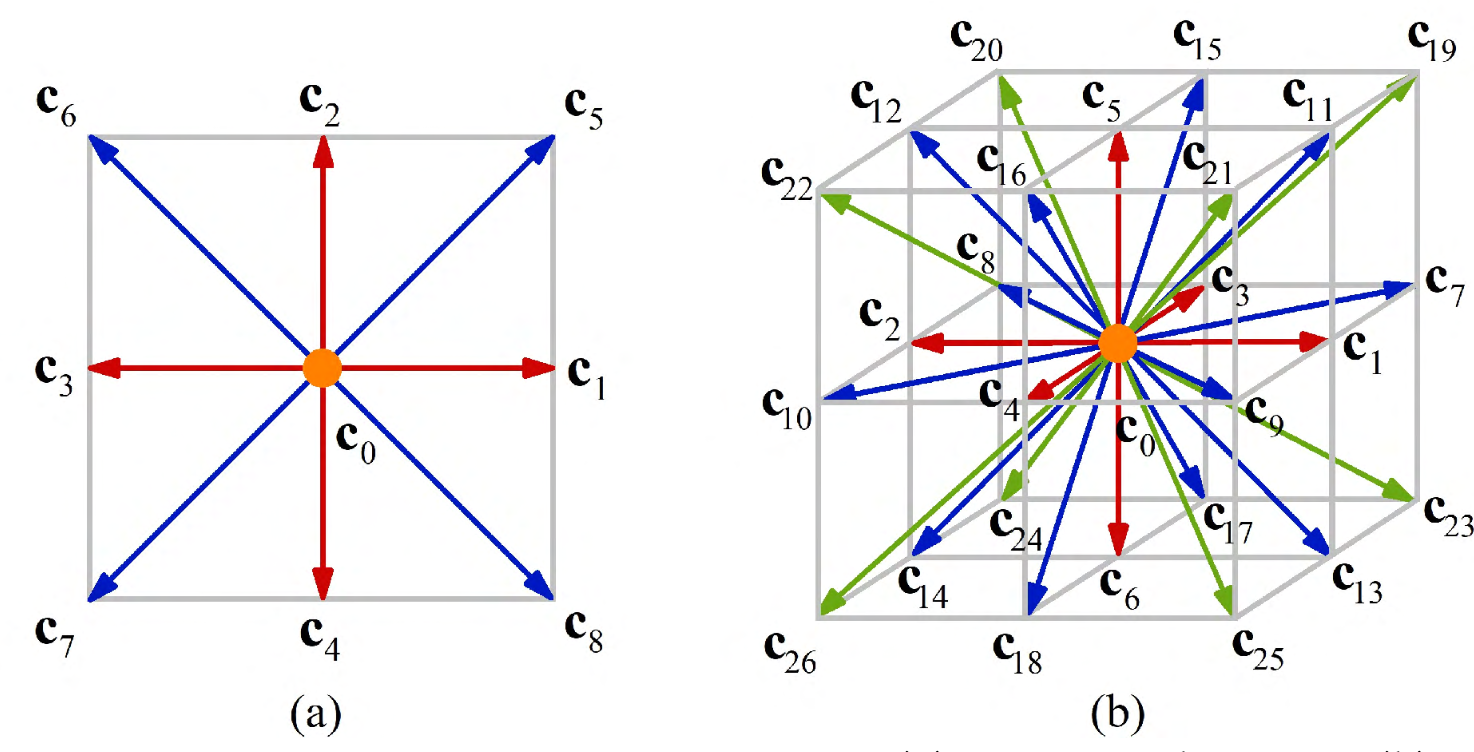
\includegraphics[width=0.6\linewidth]{lattice_figure.png}
\end{center}

There are several subtleties with this discretized velocity space, 
$\mathbb{V} \equiv \mathbb{R}^Q$. 
\begin{outline}
\1 We refer to the each microscopic velocity component with 
$f_i(x, t)$ for $i \in 0..Q - 1$.
\1 Each of these $f_i(x, t)$ values is a probability that there is a particle traveling with at a fixed velocity, $c_s$, in the direction $c_i$.
\1 Integrals over microscopic velocities can recover macroscopic properties.
In this context we refer to these integral properties as moments, 
and they are calculated as sums. 
For example, pressure and momentum (?) are the zeroth and first moment 
of the microscropic velocity distribution.
\begin{align}
  \rho(x, t) &= \sum_{i = 0}^{Q - 1} f_i(x, t) \\
  \rho(x,t)u(x,t) &= \sum_{i = 0}^{Q - 1}c_i f_i(x, t)
\end{align}
\end{outline}

 


\subsection{LBM Implementations}

There were several lattice boltzman implementations that were helpful to me.
\begin{outline}
  \1 A literate implementation of LBM using SymPy and CUDA \cite{web:literate_lbm}
  \1 An interactive 2D implementation written in Rust and WGPU \cite{web:lbm-web}.
  \2 While this was an important resource in that it demonstrated 
  the feasibility of what I wanted to do, 
  my implementation shares no code or even structural similarities 
  with this implementation.
  \1 A CPU only LBM implementation written in Rust \cite{web:lbm-rs}.
  \2 The interface and workflow of this tool was exactly what I wanted, but it didn't use the GPU at all.
  \1 An implementation of MRT LBM from \cite{Yang2022} is available on \href{https://github.com/yjhp1016/taichi_LBM3D/}{github}.
\end{outline}

WGPU on my M1 Max GPU has a max storage buffer size of $4.29$ gb.
That is sufficient to hold a billion floating point numbers.
Normally, the distributions are stored in one large contiguous allocation 
as a $D+Q$ dimensional array.
In such setup, this would limit us around $350^3$ lattice points.

By storing each direction in a separate buffer, we incur some additional expense but raise our maximum problem size to $115.83$ gb.

I opted to take on additiona

\subsection{MRT}

The multiple relaxation time collision operator (MRT),
works by first transforming transforming $f$ into moment space,
using a moment space transform $M$.
Moments show up in many contexts, but we can broadly think of them
as integral properties of $f$ \cite{Taber2018}.
MRT then can relax each moment at a separate rate, using a diagonal matrix $R$.
Finally, MRT uses $M^{-1}$ to transform the relaxed moments
back into lattice distributions. We define MRT below \cite{De2017}.
$$
\text{MRT}(f) = M^{-1} \cdot R \cdot M (f_{\text{eq}} - f)
$$
Notably, $M$ and $R$ are constant across space ($x$) and time ($t$).
We will expand on these ideas in the next section.

\subsection{CM-MRT}\label{sec:cm-mrt}
The moment space transform $M$ used in the $MRT$ collision operator
evaluates the basis polynomials at $c_{\alpha}j$
which are centered around the origin.
As a result, the collision's frame of reference $u$ affects the 
moments of the collision.
This is a violation of \textit{Galilean invariance}.
If we instead evaluate the basis polynomials using 
$\bar{c}_{\alpha,j} = c_{\alpha, j} - u_{\alpha}$,
our moments will be normalized to the collisions reference frame $u$. 
As a result, our moment transform will now depend on $u$. \cite{De2017, De2019}.


We will refine this later, our initial definition of 
the central moments multiple relaxation time collision operator (CM-MRT) 
is
$$\label{eqn:cm_mrt_def_init}
\text{CM-MRT}_{u}(f) = M_u^{-1} R  M_u(f - feq)
$$
We will exactly define the components of this definition for our
$D3Q27$ lattice, which in turn will allow us to simplify some things.

$M_u$ is our centered moment space transform, 
a rank $27$ square matrix.
The elements of $M_u$ are defined below 
(adapted from equation 35 from \cite{Li2020Supplement}, 
and equation 9 from \cite{De2017}.)
\begin{align*}
m_{0,j} &= \{  1 \},\\
m_{1,j} &= \{  \bar{c}_{j,x} \},
m_{2,j} = \{  \bar{c}_{j,y} \},
m_{3,j} = \{  \bar{c}_{j,z} \},\\
m_{4,j} &= \{  \bar{c}_{j,x} \bar{c}_{j,y} \},
m_{5,j} = \{  \bar{c}_{j,x} \bar{c}_{j,z} \},
m_{6,j} = \{  \bar{c}_{j,y} \bar{c}_{j,z} \},\\
m_{7,j} &= \{  \bar{c}_{j,x}^2 - \bar{c}_{j,y}^2 \},
m_{8,j} = \{  \bar{c}_{j,x}^2 - \bar{c}_{j,z}^2 \}, \\
m_{9,j} &= \{  \bar{c}_{j,x}^2 + \bar{c}_{j,y}^2 + \bar{c}_{j,z}^2 \},\\
m_{10,j} &= \{ \bar{c}_{j,x} \bar{c}_{j,y}^2 + \bar{c}_{j,x} \bar{c}_{j,z}^2 \},
m_{11,j} = \{ \bar{c}_{j,x}^2 \bar{c}_{j,y} + \bar{c}_{j,y} \bar{c}_{j,z}^2 \},\\
m_{12,j} &= \{ \bar{c}_{j,x}^2 \bar{c}_{j,z} + \bar{c}_{j,y}^2 \bar{c}_{j,z} \},
m_{13,j} = \{ \bar{c}_{j,x} \bar{c}_{j,y}^2 - \bar{c}_{j,x} \bar{c}_{j,z}^2 \},\\
m_{14,j} &= \{ \bar{c}_{j,x}^2 \bar{c}_{j,y} - \bar{c}_{j,y} \bar{c}_{j,z}^2 \},
m_{15,j} = \{ \bar{c}_{j,x}^2 \bar{c}_{j,z} - \bar{c}_{j,y}^2 \bar{c}_{j,z} \},\\
m_{16,j} &= \{ \bar{c}_{j,x} \bar{c}_{j,y} \bar{c}_{j,z} \},\\
m_{17,j} &= \{ \bar{c}_{j,x}^2 \bar{c}_{j,y}^2 + \bar{c}_{j,x}^2 \bar{c}_{j,z}^2 + \bar{c}_{j,y}^2 \bar{c}_{j,z}^2 \},\\
m_{18,j} &= \{ \bar{c}_{j,x}^2 \bar{c}_{j,y}^2 + \bar{c}_{j,x}^2 \bar{c}_{j,z}^2 - \bar{c}_{j,y}^2 \bar{c}_{j,z}^2 \}, \\
m_{19,j} &= \{ \bar{c}_{j,x}^2 \bar{c}_{j,y}^2 - \bar{c}_{j,x}^2 \bar{c}_{j,z}^2 \},\\
m_{20,j} &= \{ \bar{c}_{j,x}^2 \bar{c}_{j,y} \bar{c}_{j,z} \},
m_{21,j} = \{ \bar{c}_{j,x} \bar{c}_{j,y}^2 \bar{c}_{j,z} \},\\
m_{22,j} &= \{ \bar{c}_{j,x} \bar{c}_{j,y} \bar{c}_{j,z}^2 \},\\
m_{23,j} &= \{ \bar{c}_{j,x} \bar{c}_{j,y}^2 \bar{c}_{j,z}^2 \},
m_{24,j} = \{ \bar{c}_{j,x}^2 \bar{c}_{j,y} \bar{c}_{j,z}^2 \},\\
m_{25,j} &= \{ \bar{c}_{j,x}^2 \bar{c}_{j,y}^2 \bar{c}_{j,z} \},\\
m_{26,j} &= \{ \bar{c}_{j,x}^2 \bar{c}_{j,y}^2 \bar{c}_{j,z}^2 \},\\
\end{align*}

To define our relaxation rates, $R$, we need to address
the specific meaning of our moment space.
We have $27$ moments, $m_j$.
$m_0$ is mass density $\rho$, 
$m_1, m_2, m_3$ represent the components of momentum.
$m_4$ through $m_9$ are the second order moments related
to momentum flux.
The first $9$ moments have physical interpretations,
and their relaxation rates follow \cite{Li2020, De2017}.
\begin{align}
  r_0 &= 0, \nonumber \\
  r_i &= 2, \text{ for } i = 1,2,3 \nonumber \\
  r_i &= (3v + 1 / 2)^{-1}, \text{ for } i = 4,\ldots, 9 \label{eqn:kv_rate}
\end{align}
Setting the relaxation rates for higher order moments 
is an area of active research.
In \cite{Li2020} an adaptive scheme for updating these rates
over time was described.
We didn't attempt to implement that, 
and instead utilized the constant rates proposed in \cite{Li2018}.
They suggest using following viscosities for
to use with equation \ref{eqn:kv_rate}
for the higher order relaxation rates. 
\begin{align*}
  v_i &= 0.005, \text{ for } i = 9,\ldots, 16 \\
  v_i &= 0.007, \text{ for } i = 17, \ldots, 22 \\
  v_i &= 0.009, \text{ for } i = 26 
\end{align*}

Lastly, we need to revisit $f_{\text{eq}}$.
We utilize a full sixth order Hermite expansion for 
equilibrium function, as proposed in \cite{Shan2006}.
This expansion is quite complex, but it has an elegant
representation in centralized moment space.
Most entries in $M_u f_{\text{eq}} = \bar{m}$ are zero, 
except for
$$
\bar{m}_0 = \bar{m}_9 = \rho, \bar{m}_{17} = c_s^2 \rho, \bar{m}_{18} = c_s^4\rho \bar{m}_{26} = c_s^6 \rho
$$
Notably, our equilibrium moments in this space only depend on $\rho$,
and not $u$, which demonstrates Galilean invariance.

We can not present the final definition of CM-MRT that we implemented.
\begin{align}
  \text{CM-MRT}(f) = M_u^{-1} R (M_u f - \bar{m}) \label{eqn:cm-mrt}
\end{align}

CM-MRT is a challenge to implement by hand, 
as $M_u, M_u^{-1}, \bar{m}$ must be derived at every evaluation.
Additionally, many GPU frameworks
don't have a sufficiently advanced linear algebra package available
to directly express equation \ref{eqn:cm-mrt}.
Code generation using a computer algebra system is a technique used 
in \textit{lbmpy} \cite{Hennig2023}, 
and \textit{A Literate Lattice Boltzmann Code} \cite{web:literate_lbm} 
to generate shader code that
evaluates collision operators.

\subsection{Zero-centered Storage}
LBM is very sensitive to floating point error.
An important technique for mitigating these errors is 
\textit{zero-centered storage} \cite{Lehmann2022, Hennig2023}.

